\section{Méthodologie Agile}\label{sec:agile}

L'équipe de développement de la géolocalisation de SuiviDeFlotte -- comme les autres équipes de développement de l'entreprise -- travaille selon la méthodologie agile SCRUM. Cette méthodologie est une approche de gestion de projet qui met l'accent sur la flexibilité, la collaboration et la livraison continue. Elle est largement utilisée dans le développement de logiciels et peut également être appliquée à d'autres domaines. SCRUM divise un projet en cycles appelés ``itérations'' ou ``sprints'' de courte durée, généralement de deux à quatre semaines, pendant lesquels une partie du travail est accomplie et livrée.

Les termes clés de la méthodologie SCRUM sont énumérés ci-dessous et illustrés dans la Figure~\ref{fig:agile}.

\begin{description}
    \item[Product Owner (Propriétaire du Produit)] La personne responsable de définir et de prioriser les éléments du produit à développer. Le Propriétaire du Produit représente les besoins des utilisateurs et des parties prenantes.
    \item[Scrum Master (Maître de Scrum)] Le facilitateur du processus SCRUM. Le Scrum Master s'assure que l'équipe suit les principes SCRUM, élimine les obstacles et favorise un environnement de travail efficace.
    \item[Équipe de Développement] Le groupe de professionnels chargé de concevoir, développer, tester et livrer les éléments du produit à la fin de chaque sprint.
    \item[User Story (Histoire Utilisateur)] Une Histoire Utilisateur est une courte description d'une fonctionnalité ou d'un aspect du produit, racontée du point de vue de l'utilisateur. Elle suit généralement le format ``En tant que [utilisateur], je veux [action] afin de [objectif]''. Les Histoires Utilisateurs sont des éléments du Carnet de Produit et aident à définir les fonctionnalités du produit du point de vue de l'utilisateur.
    \item[Story Point (Point d'Histoire)] Le Point d'Histoire est une unité relative utilisée pour estimer la complexité, l'effort et la taille des Histoires Utilisateurs ou des tâches de développement. Il n'a pas de valeur absolue, mais il sert à comparer la difficulté relative entre différentes Histoires Utilisateurs. Les équipes de développement attribuent des points d'histoire lors des estimations, ce qui les aide à planifier la quantité de travail qu'elles peuvent accomplir dans un sprint donné.
    \item[Epic (Épique)] Un Épic est une unité de travail plus large que les Histoires Utilisateurs individuelles. Il représente généralement un ensemble de fonctionnalités, de tâches ou de travaux qui sont trop importants pour être traités dans un seul sprint. Les Épics sont souvent des objectifs à long terme qui sont décomposés en Histoires Utilisateurs plus petites et gérables. Ils aident à organiser et à structurer le développement du produit en regroupant des éléments liés autour d'un thème ou d'un objectif commun. Les Épics sont inclus dans le Carnet de Produit et sont priorisés en fonction de leur valeur pour l'utilisateur et du contexte global du projet.
\end{description}

SCRUM encourage la transparence, l'adaptabilité et la collaboration continue entre les membres de l'équipe et les parties prenantes, ce qui permet de s'adapter aux changements et de fournir rapidement de la valeur tout au long du projet.

\begin{figure}[h]
    \centering
    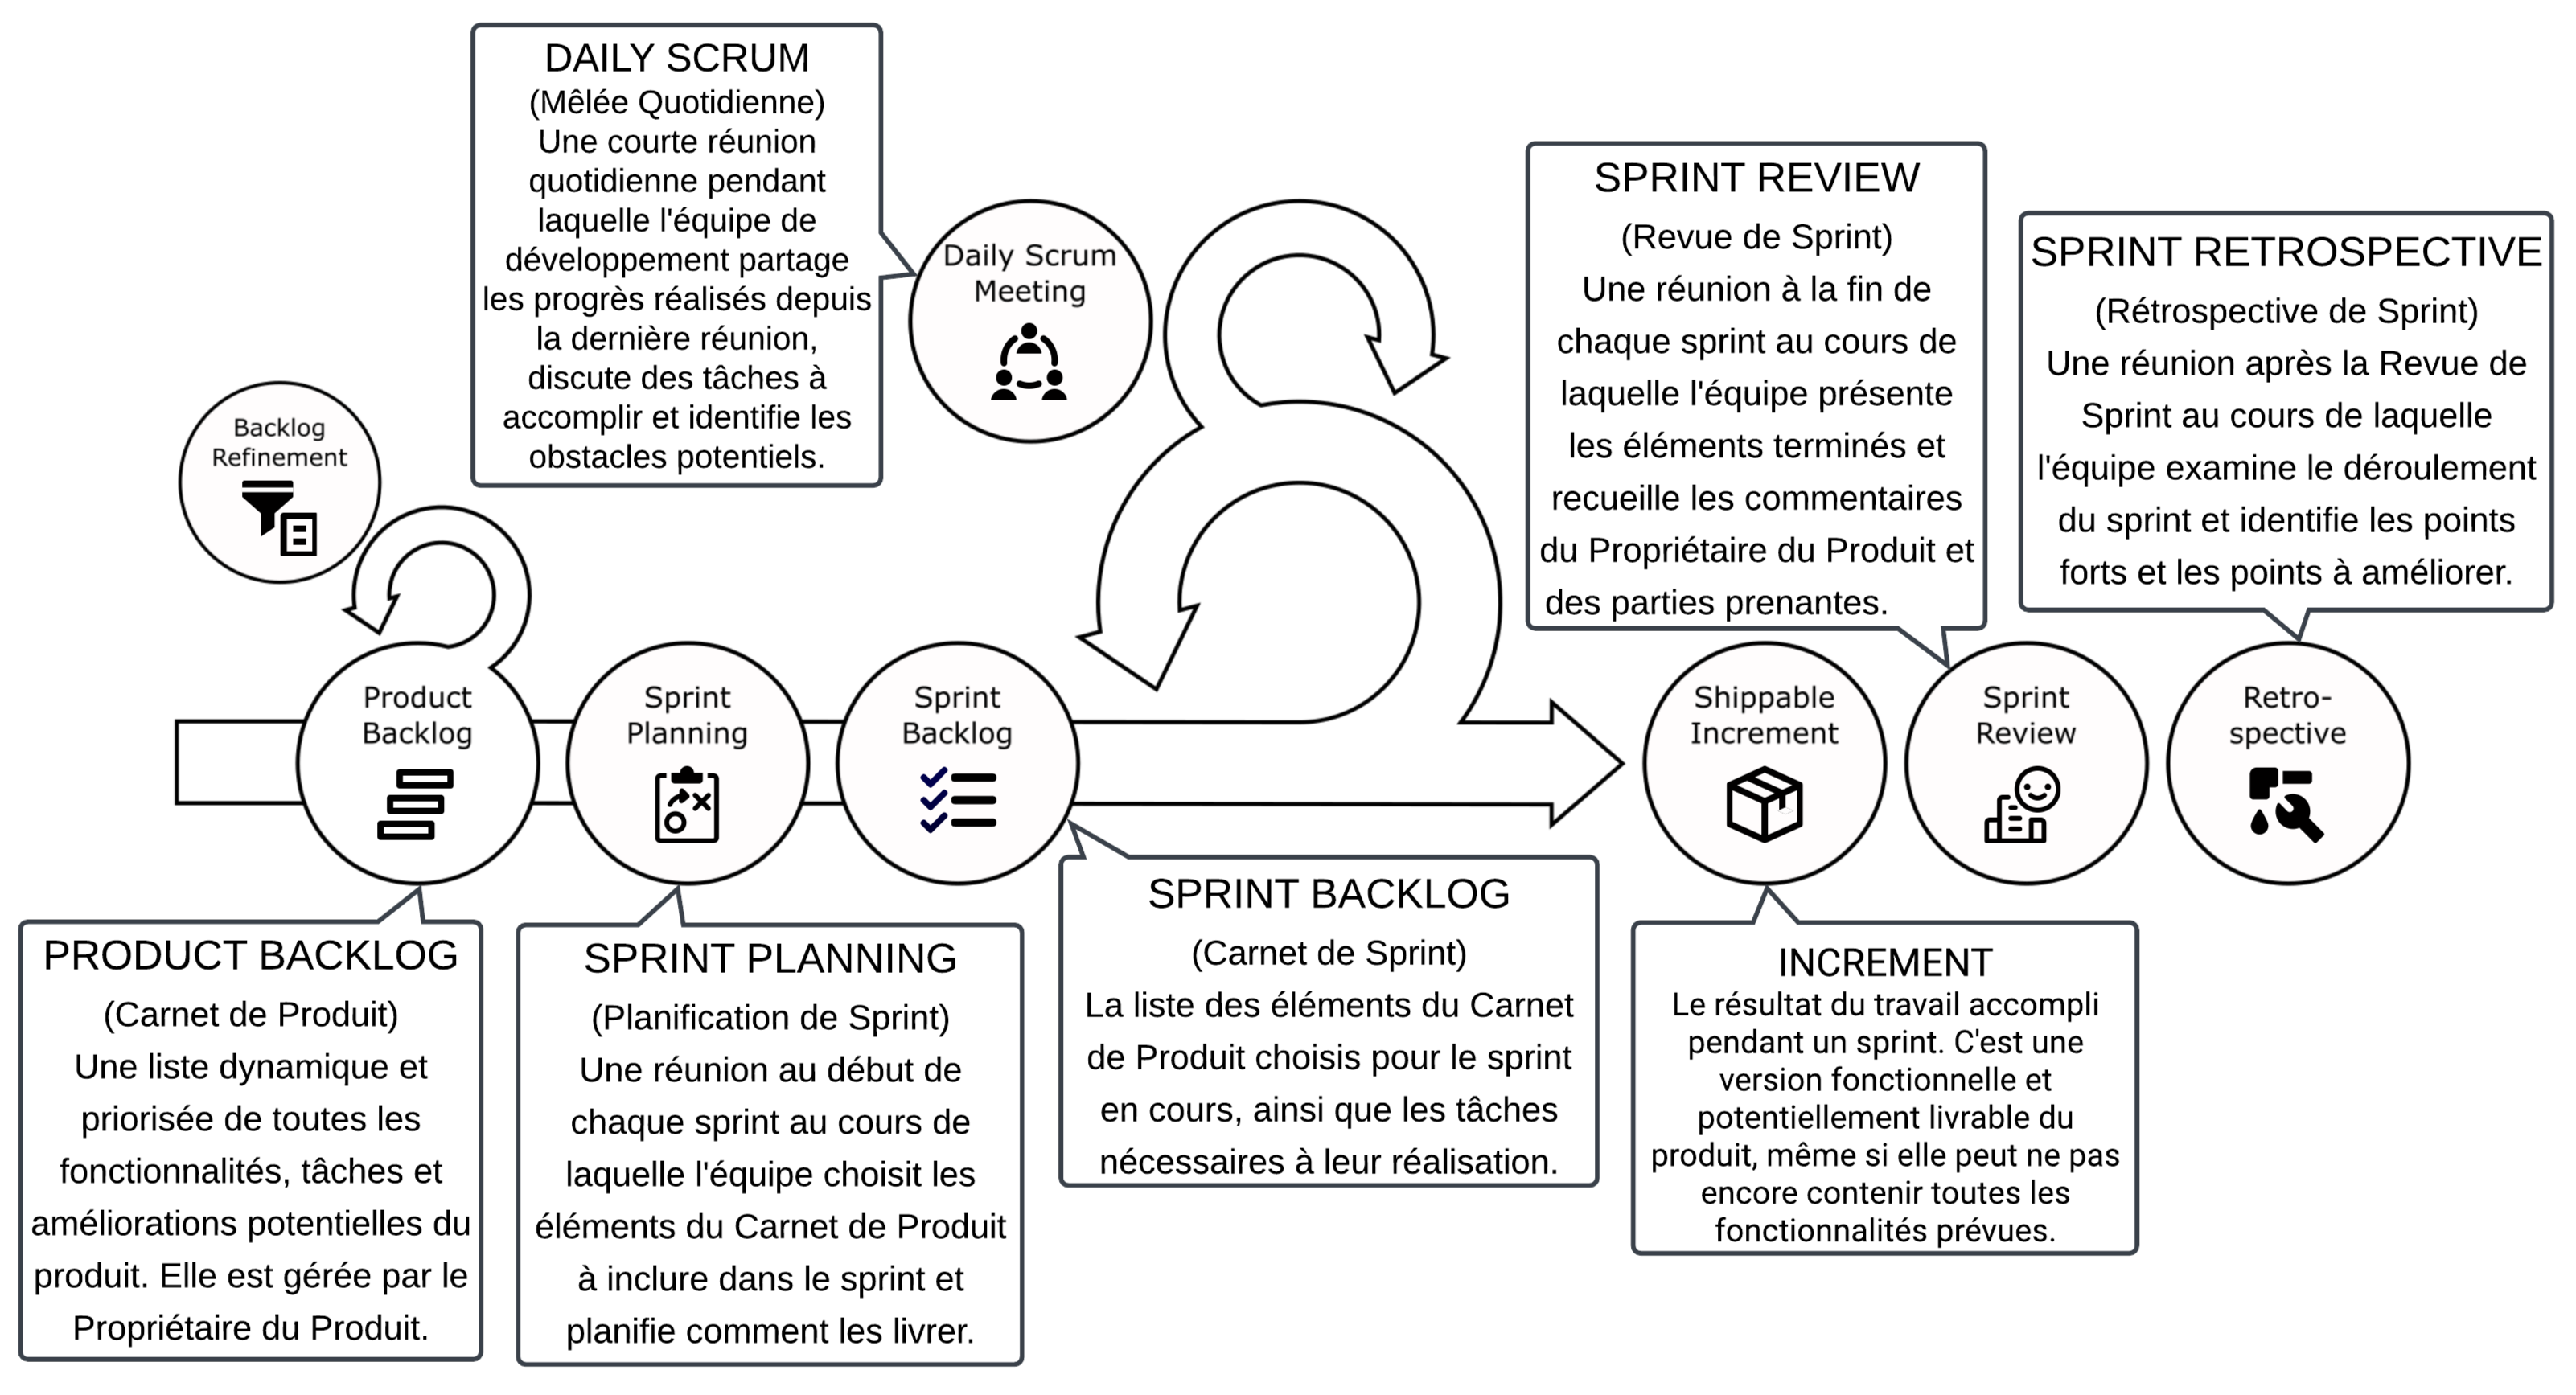
\includegraphics[width=\textwidth]{img/agile-02}
    \caption{Cérémonies SCRUM.}
    \label{fig:agile}
\end{figure}

Dans l'équipe Géoloc, le processus suit un calendrier de sprints de deux semaines (Figure~\ref{fig:sprint}). Chaque cycle commence par un ensemble de réunions clés qui ont lieu tous les deuxièmes mardis. Cette journée englobe la Revue de Sprint, la Rétrospective de Sprint et la Planification de Sprint. Lors de la Revue de Sprint, les éléments achevés sont présentés au Propriétaire du Produit et aux parties prenantes, les retours sont recueillis et les priorités sont ajustées si nécessaire. La Rétrospective de Sprint offre l'opportunité à l'équipe de réfléchir aux succès et d'identifier les domaines à améliorer, favorisant une culture d'amélioration continue. Ensuite, la Planification de Sprint implique la sélection des Histoires Utilisateurs du Carnet de Produit à inclure dans le sprint à venir, en tenant compte de leur complexité et de leur priorité. Pour l'estimation de la complexité des tâches, des Points d'Histoire basés sur la séquence de Fibonacci (1, 2, 3, 5, 8, 13) sont utilisés. Cette approche aide à attribuer des valeurs relatives à différentes tâches et assure une évaluation cohérente de la charge de travail.

À la fin de chaque sprint, les nouveaux incréments sont également mis en production. Grâce à l'approche Agile et à la fréquence des mises en production, les modifications apportées à l'application sont rapidement portées à la connaissance de l'utilisateur.

Chaque jour ouvrable débute par une Mêlée Quotidienne de 15 minutes, au cours de laquelle les progrès depuis la dernière réunion sont passés en revue, les tâches sont discutées et les obstacles potentiels sont identifiés. Ces réunions se déroulent généralement en ligne via Google Meet pour accueillir les collègues travaillant à distance et garantir la participation de tous les membres de l'équipe, peu importe leur emplacement. Par contre, pour maintenir la communication et la cohésion de l'équipe, les réunions du mardi de chaque deuxième semaine sont des réunions en personne. Cette pratique encourage les échanges directs, la collaboration étroite entre les membres de l'équipe et facilite la résolution rapide de tout problème ou obstacle pouvant survenir.

\begin{figure}[h]
    \centering
    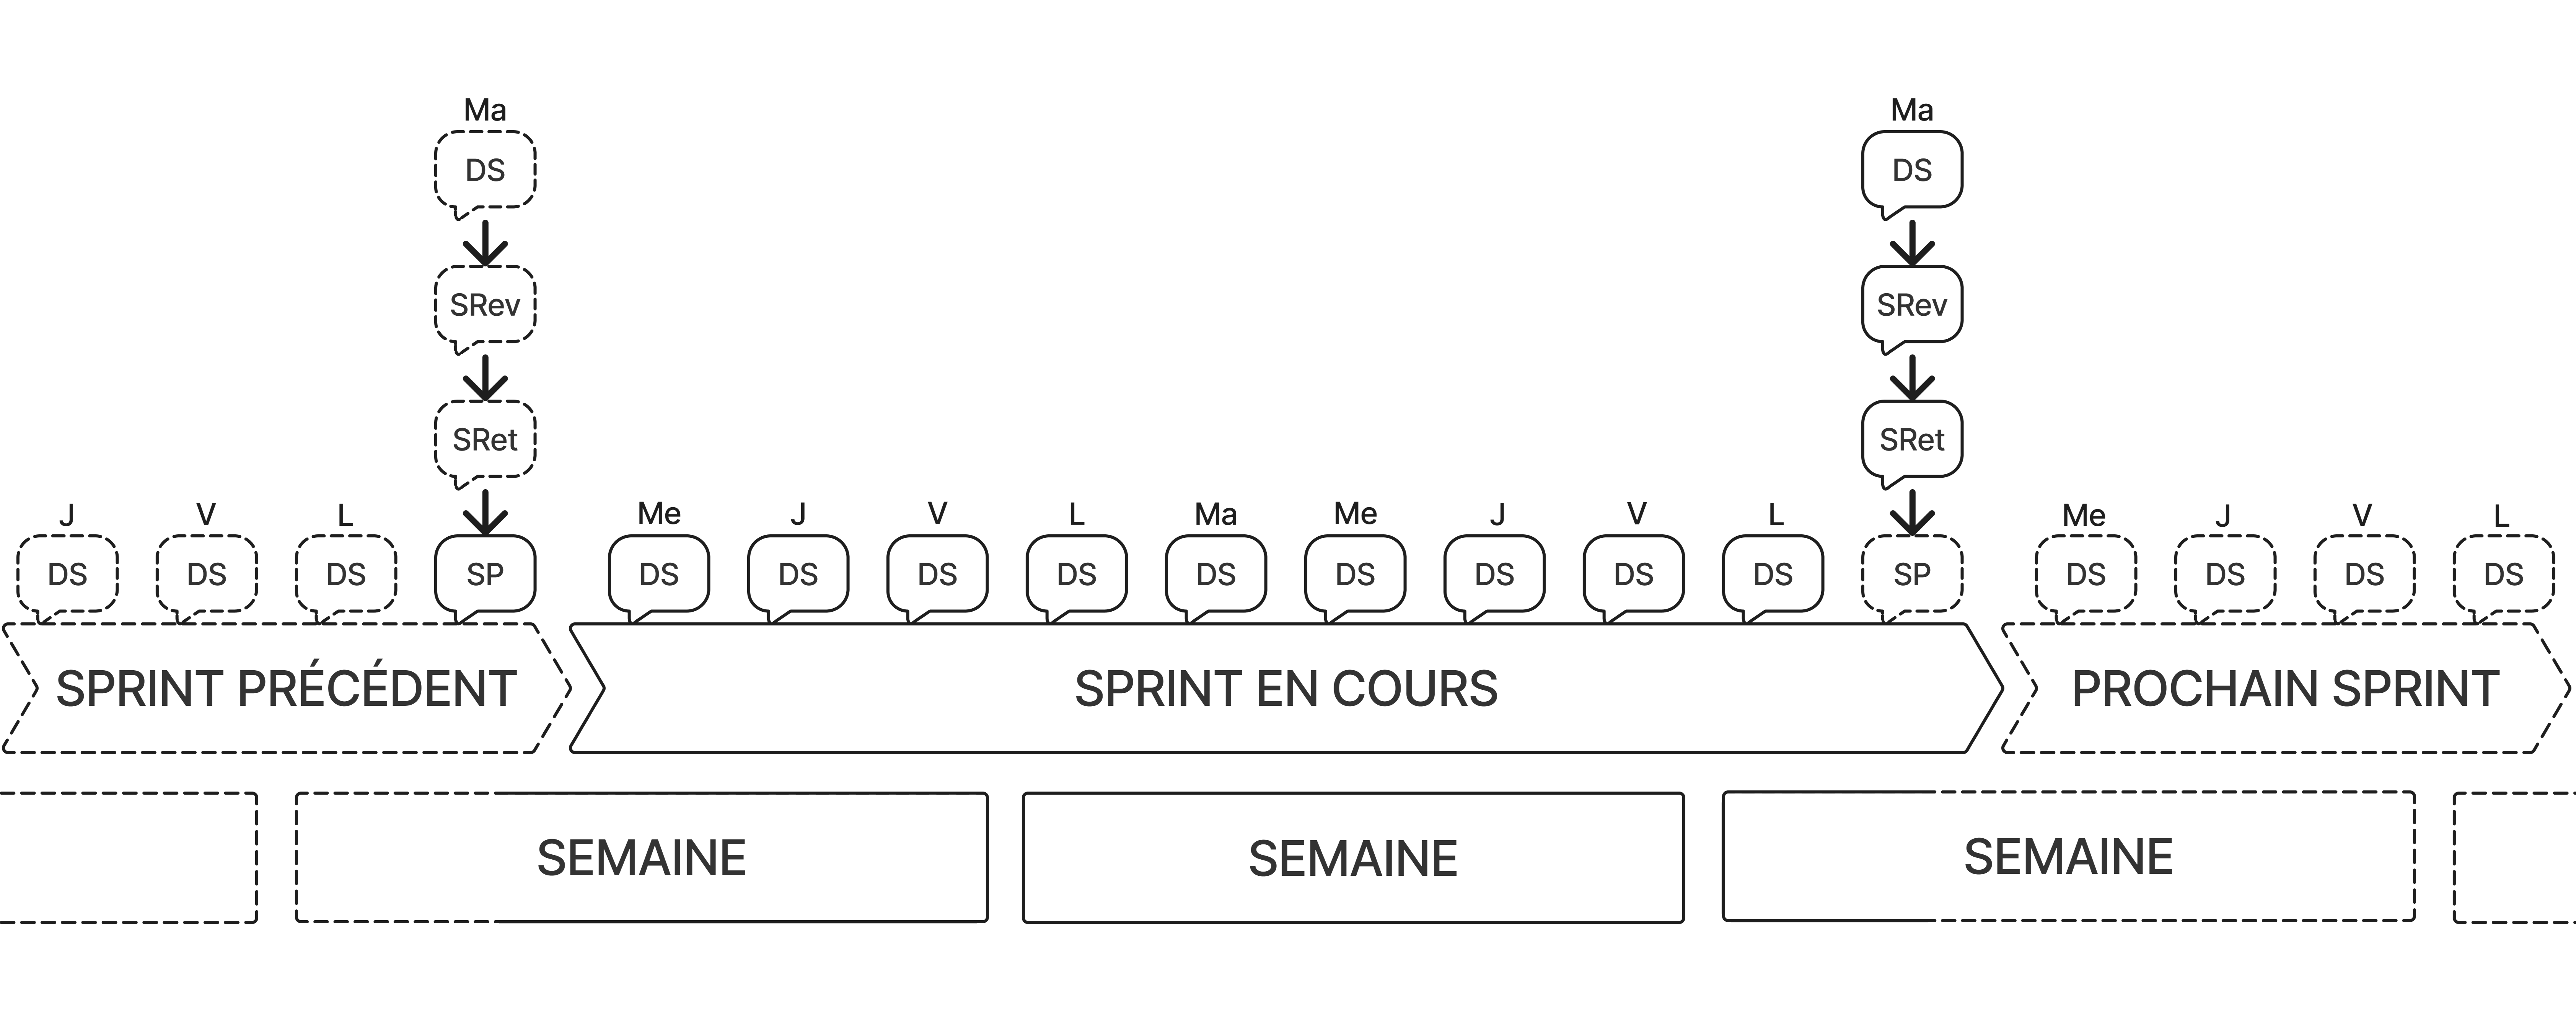
\includegraphics[width=\textwidth]{img/sprint04}
    \caption{Programme des sprints chez SuiviDeFlotte. Légende : L, Ma, Me, J, V -- jours de la semaine ; DS -- Daily Scrum ; SRev -- Sprint Review ; Sret -- Sprint Retrospective ; SP -- Sprint Planning ; ligne pointillée -- Sprint précédent ou suivant ; ligne continue -- Sprint en cours.}
    \label{fig:sprint}
\end{figure}

Actuellement, les rôles du Propriétaire du Produit et du Maître de Scrum ont été temporairement fusionnés en une seule personne. Cette configuration permet au Propriétaire du Produit de gérer les responsabilités du projet tout en facilitant le processus SCRUM, en maintenant une communication fluide avec l'équipe de développement.

En complément des cycles de deux semaines des Sprints, l'opération de l'entreprise comprend également un cycle plus long. En effet, comme je l'ai mentionné dans l'introduction de ce chapitre, l'entreprise publie une nouvelle version, appelée nouvelle Edition, de ses services en ligne tous les quatre mois, soit trois fois par an. Cela implique qu'il y a environ huit sprints pour que les développeurs puissent concevoir les nouvelles fonctionnalités des nouvelles éditions.

La Figure~\ref{fig:committees-and-scrum} résume les relations entre les comités et le processus des sprints.

\begin{figure}[h]
    \centering
    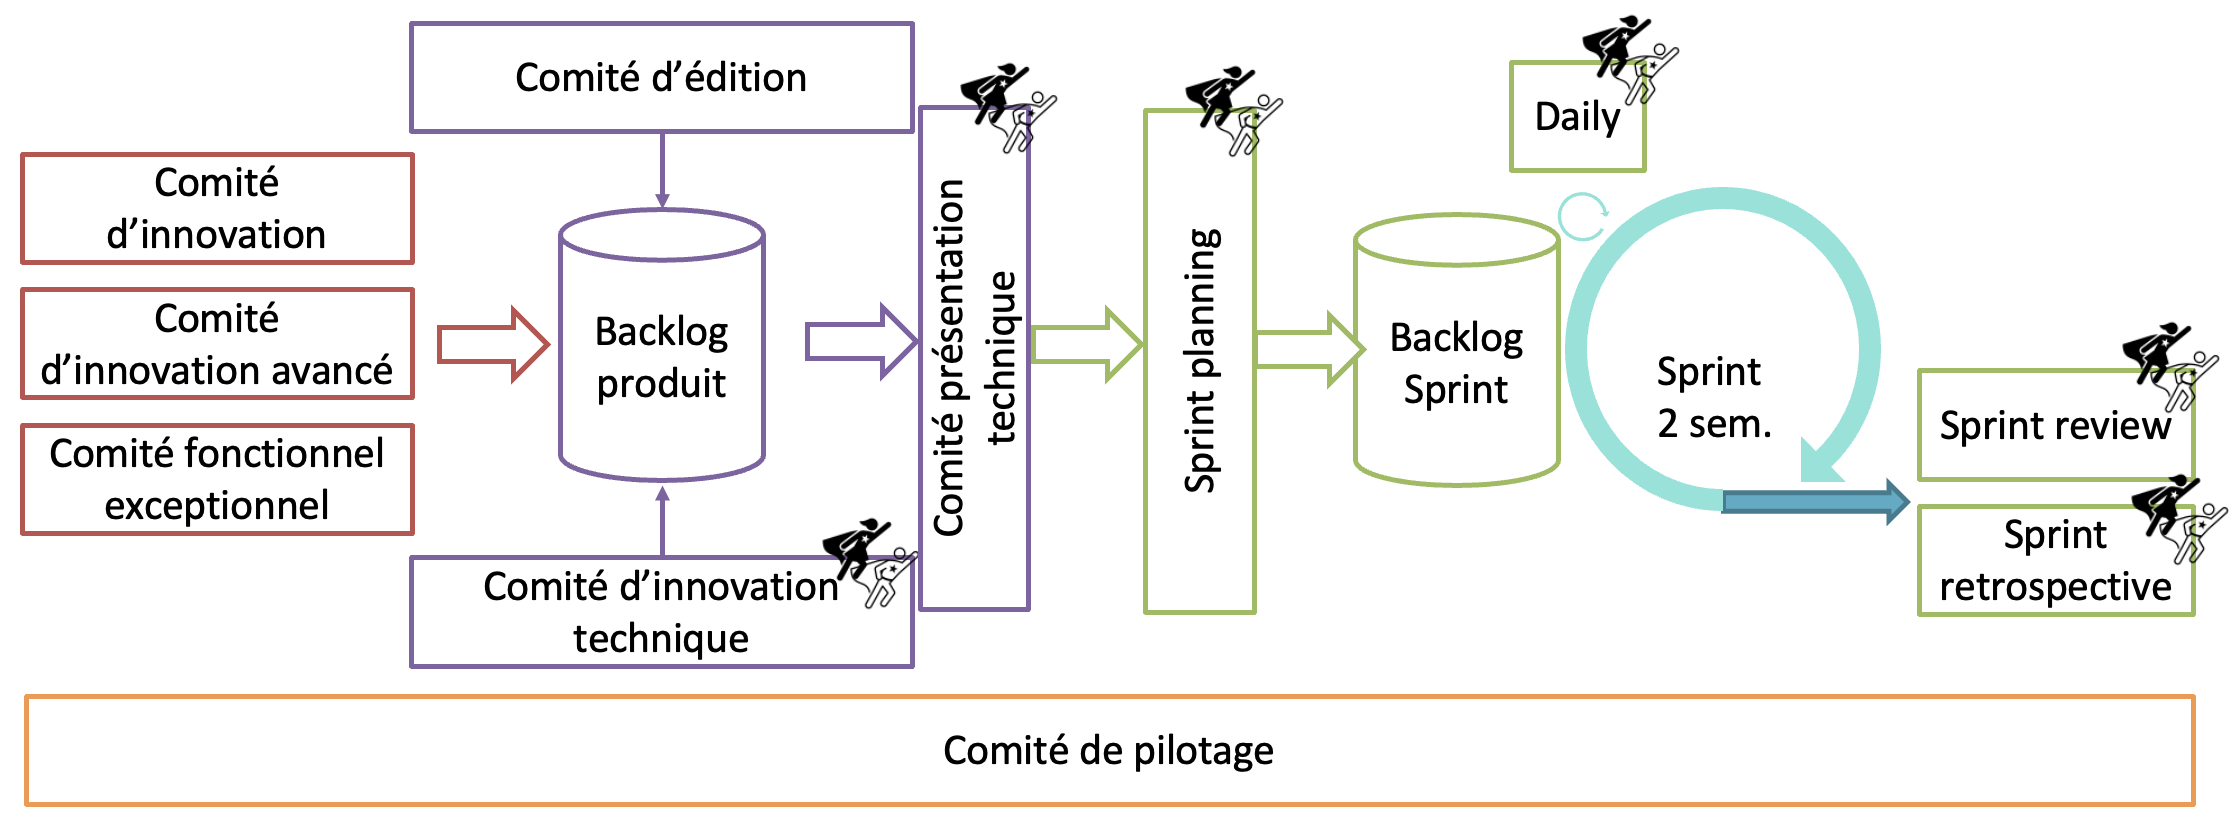
\includegraphics[width=\textwidth]{img/committees-and-scrum}
    \caption{Résumé des relations entre les comités et le processus des sprints.}
    \label{fig:committees-and-scrum}
\end{figure}